%% -*- mode: LaTeX; compile-command: "mk" -*-

\newpage
\chapter*{Acknowledgments}

During the first few years of my PhD, I floundered around among
various research topics, trying to find one that I could get truly
excited about. I even wondered at times whether I made a mistake in
choosing an advisor.  In retrospect, I can say with confidence that I
did not! Despite the fact that we have fairly different interests and
different approaches to research, Stephanie Weirich has been a
wonderful advisor.  She has always encouraged me to pursue my
passions, even to the point of allowing me to take on a dissertation
topic she knew very little about.  Perhaps most importantly, she has
done a masterful job getting me to actually graduate (no mean
feat)---by turns encouraging and challenging me, each at the
appropriate moment.

Jacques Carette has been an unofficial second advisor to me.  Despite
having plenty of ``official'' advisees also demanding his time and
attention, he has generously taken the time to collaborate, give
feedback and advice, and even twice to host me for a week of focused,
face-to-face collaboration.  This dissertation literally would not
exist were it not for his academic and personal generosity, for which
I will always be grateful.

My family has been, and continues to be, a constant source of joy and
encouragement.  My wife and bestest friend Joyia, more than anyone
else, is the one who encouraged me through the darkest points and
convinced me to keep going.  She has also sacrificed much in order to
give me the time and space necessary to finish. My son Noah, too, has
sacrificed---in ways he doesn't even understand---while his daddy
wrote a ``very long story about computers and numbers''.  But I could
always count on him to cheer me up with tickle fights.

The other members of the Penn programming languages group---especially
(though by no means limited to) Chris Casinghino, Richard Eisenberg,
Nate Foster, Michael Greenberg, Peter-Michael Osera, Benjamin Pierce,
Vilhelm Sj\"oberg, Daniel Wagner, and Steve Zdancewic---deserve a
great deal of thanks for all their support over the years, through
moral support and encouragement, critical feedback on papers and
talks, enlightening discussions, and simply friendship.  PL Club has
been a wonderfully collegial community in which to learn and work.

While developing the ideas in this dissertation I have benefited over
the years, both directly and indirectly, from conversations with many
people in the Haskell community and the wider FP and PL communities,
particularly Faris Abou-Saleh, Reid Barton, Gershom Bazerman, Conal
Elliott, Jeremy Gibbons, Andy Gill, Jason Gross, Ralf Hinze, Neel
Krishnaswami, Dan Licata, Peter Lumsdaine, Simon Peyton Jones, Ross
Street, Andrea Vezzosi, and Nick Wu, along with many others.  I am
also grateful to Heinrich Apfelmus, Toby Bartels, Shachaf Ben-Kiki, Gabor Greif, Jay
McCarthy, Colin McQuillan, David Roberts, Jon Sterling, and Ryan
Yates, all of whom read early drafts of this dissertation and sent me
typo reports as well as more substantial suggestions, greatly
improving the final product.  Thanks also to the anonymous MSFP and
MFPS reviewers, whose feedback on submissions based on this material
led to many substantial improvements to the technical content.

The \texttt{diagrams} community---particularly Daniel Bergey, Chris
Chalmers, Allen Gardner, Niklas Haas, Claude Heiland-Allen, Chris
Mears, Jeff Rosenbluth, Carter Schonwald, Michael Sloan, Luite
Stegeman, and Ryan Yates---has been a great source of joy to me during
the long process of completing my PhD.  Not only have they provided
encouragement, camaraderie, and welcome distraction, but this
dissertation itself is richer for their contributions to
\texttt{diagrams}---many of the diagrams throughout this document make
nontrivial use of features contributed by other members of the
community.  It has also been a particular joy to see the project
continue humming along even during my virtual absence while writing.

It is staggering to consider the wealth of relationship accumulated
during six years at City Church Philadelphia.  I particularly thank
Tuck and Stacy Bartholomew, Darren Bell, Dave and Katie Brindley, Zac
and Joanna Brooks, Sara Cayless, Mike and Sonja Chen, Tim and Ruth
Creber, Chris and Bonnie Currie, Ben Doane and Melissa McCarten, John
Dyck, Will and Margaret Kendall, Dick Landis, Colin and Lauren
Marlowe, Drew and Susie Matter, Nick McAvoy, Chris and Sarah Miciek,
Jeremy Millington, Cat Ricketts, Ben Smith, Josh and Kory Stamper, Ben
Sykora and Beth Dyson, Matt Thanabalan and Carrie Lutjens, Gene and
Laura Twilley, and Jackson Warren, all of whom, at various times and
in various ways, have provided encouragement and support as I made my
way through graduate school. It is certain that I have forgotten
others who should also be on this list, and in any case it is not even
clear where the list should stop!

I thank the Mustard Seed Foundation for their affirmation in selecting
me as a Harvey Fellow, and for their support, both financially, and in
helping me think through the integration of my faith and work.

A heartfelt thank you to the Williams College computer science
department for the genuine care and support I have received as a
visiting faculty member, and especially to Bill Lenhart for his
generous gift of time in taking on most of the grungy legwork for CS
134.  Beginning a new job, teaching two classes, and simultaneously
completing a dissertation would be impossible even to contemplate were
it not undertaken in such a supportive environment.

In Philadelphia, the Green Line Cafe, Lovers \& Madmen, the Penn
Graduate Student Center, and Van Pelt library---and in Williamstown,
Tunnel City Coffee and the Schow science library---have all provided
wonderfully conducive environments for focused writing sessions.

Last but certainly not least, a big thank you is due to Beeminder
(\url{http://beeminder.com}), and to its cofounders, Bethany Soule and
Danny Reeves.  The chance that I would have successfully finished this
dissertation without Beeminder is vanishingly small, for the simple
reason that a dissertation cannot be put off until a week before it is
due.  \$145 for the motivation to write a dissertation is quite a
steal; I owe the whole Beeminder team a round of beers!

\begin{center}
  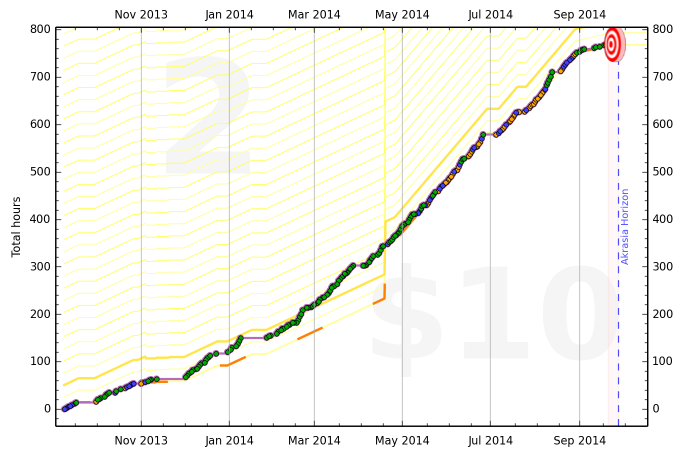
\includegraphics[width=4in]{thesis-beeminder}
\end{center}

Finally, my work has been supported by the National Science
Foundation under the following grants:
\begin{itemize}
\item NSF 1218002, CCF-SHF Small: \emph{Beyond Algebraic Data Types:
  Combinatorial Species and Mathematically-Structured Programming}
\item NSF 1116620, CCF-SHF Small: \emph{Dependently-typed Haskell}
\item NSF 0910500, CCF-SHF Large: \emph{Trellys: Community-Based
    Design and Implementation of a Dependently Typed Programming
    Language}
\end{itemize}
and by the Defense Advanced Research Projects Agency under the
following grant:
\begin{itemize}
\item DARPA Computer Science Study Panel Phase
  II. \emph{Machine-Checked Metatheory for Security-Oriented
    Languages.}
\end{itemize}

\subsection*{Statement of contribution}

Parts of \pref{chap:species}, particularly the enumeration of
categorical properties needed to support various species operations,
were carried out in collaboration with Jacques Carette.  The rest of
this dissertation is my own original work.
